\subsection{You Only Look Once}

Der Algorithmus \textit{You Only Look Once} (YOLO) ist ein weiterer Objekterkennungsalgorithmus und betrachtet statt separaten Bildregionen das komplette Bild. Er benutzt nur ein neuronales Netz, um Bounding Boxen und Wahrscheinlichkeiten für bestimmte Klassen vorherzusagen.

Hierzu wird ein \textit{S x S} Gitter über das Bild gelegt. Für jedes Feld in dem Gitter werden \textit{B} Bounding Boxen erzeugt. Jede Box besitzt neben den zum Gitterfeld relativen Positionswerten einen Wert für die Vorhersage der jeweiligen Klasse. Dieser Wert wird als \textit{confidence score} bezeichnet und wird durch die Multiplikation der Wahrscheinlichkeit für ein Objekt innerhalb der Box mit der \textit{Intersection over Union} (IoU) berechnet. Die IoU bildet die Präzision der berechneten Box im Verhältnis zu der Box aus den vortrainierten Testdaten. \cite[S. 2]{JosephRedmon.2016} 

Aus der Menge an Bounding Boxen werden schließlich mit Hilfe eines festgelegten Schwellwertes die Boxen mit gefundenen Objekten bestimmt (siehe Abbildung \ref{yolo_model}).

\begin{figure}[ht]
	\begin{center}
		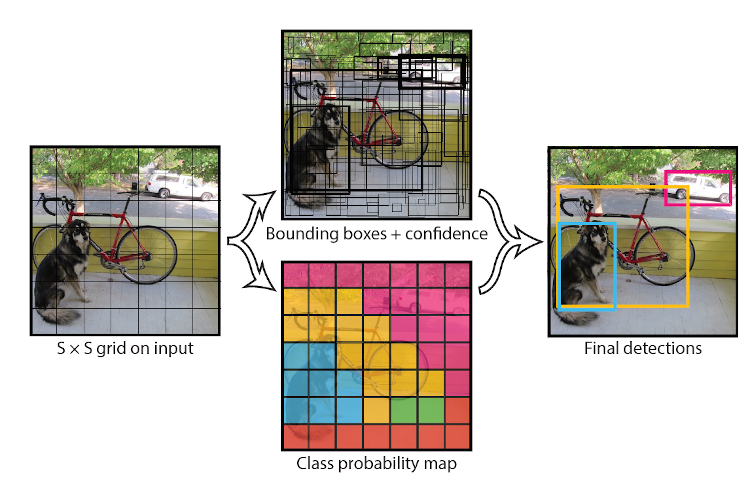
\includegraphics[width=12cm]{Bilder/yolo_model.png} 
		\caption{Vereinfachte Darstellung der Objekterkennung mit dem YOLO Algorithmus \cite[S. 2]{JosephRedmon.2016}}
		\label{yolo_model}
	\end{center}
\end{figure}

\subsubsection{YOLOv2}

\subsubsection{YOLOv3}




